\capitulo{Técnicas y herramientas}
\label{cha:Técnicas y herramientas}

En el área de la inteligencia artificial, y en general en la informática, la
conocida expresión <<Pararse a hombros de gigantes>> tiene mucho sentido, ya que
es muy difícil, y contraproducente, crear algo por completo desde cero, siempre
se utilizan herramientas, librerías o frameworks (abstracciones en general)
creados por otras personas para acelerar el trabajo y permitir que al
programador centrarse en la lógica de negocio que quiere implementar.

Este capítulo enumera las técnicas y herramientas de otras personas que se han
utilizado durante la realización de este proyecto.

\section{Técnicas}

Esta sección detalla las distintas técnicas que fueron utilizadas durante el
desarrollo de este proyecto.

\subsection{CRISP-DM}

<<Cross-industry standard process for data mining>>, conocido como (CRISP-DM),
es un modelo estándar abierto del proceso que describe los enfoques comunes que
utilizan los expertos en minería de datos \cite{shearer2000crisp}. Este estándar
surgió a finales de los 90 a partir de la inexistencia y necesidad de un enfoque
ampliamente aceptado para la minería de datos. Para conseguir esto, CRISP-DM es
agnóstico a la industria y herramientas que se utilicen, lo que permite que sea
utilizado en un amplio abanico de situaciones, lo que facilitó su adopción.

CRISP-DM divide el ciclo de vida de un proyecto de minería de datos en las
siguientes 6 fases.

\begin{enumerate}
    \item \textbf{Entendimiento del negocio}: La fase más importante de
    cualquier proyecto de minería de datos, consiste en obtener un entendimiento
    sobre los objetivos del proyecto desde el punto de vista del negocio y
    redefinir estos objetivos como un problema de minería de datos diseñado para
    cumplir con estos objetivos.
    \item \textbf{Entendimiento de los datos}: La fase de entendimiento de datos
    comienza con una recolección inicial de datos. A continuación, se procede a
    analizar los datos para obtener cierta familiaridad con los mismos,
    identificar problemas y realizar hipótesis iniciales sobre la información
    oculta que pueda existir.
    \item \textbf{Preparación de los datos}: La fase de preparación de los datos
    cubre todas las actividades realizadas para la construcción del conjunto de
    datos final a partir de la información sin procesar que se va a utilizar
    para entrenar los modelos de aprendizaje. Esta fase incluye la selección,
    limpieza, integración y formateado de los datos.
    \item \textbf{Modelado}: En esta fase se seleccionan varios algoritmos de
    aprendizaje, cuyos parámetros deben ser calibrados para ajustarse al
    conjunto de datos de forma óptima. Diferentes algoritmos imponen diferentes
    requisitos sobre el conjunto de datos sobre el que puede trabajar, por lo
    que es posible que se deba volver a la fase anterior para reajustar el
    conjunto de datos final. Esta fase incluye la selección de los algoritmos a
    utilizar, la creación de los modelos y la evaluación del rendimiento de los
    mismos.
    \item \textbf{Evaluación}: Antes del despliegue del modelo final es de gran
    importancia reevaluar si el modelo cumple realmente con los objetivos de
    negocio establecidos en la primera fase. Aquí se deberá determinar cómo se
    van a utilizar los resultados de la minería de datos. Los procesos clave de
    esta fase son la evaluación de los resultados, la revisión del proceso
    utilizado y la determinación de los pasos siguientes.
\end{enumerate}

Las fases anteriores tienen una naturaleza cíclica, los conocimientos obtenidos
en cada ciclo de CRISP-DM se utilizan para replantear los objetivos de negocio y
repetir el proceso con los nuevos conocimientos. Como muestra la siguiente
figura.

\begin{figure}[!h]
      \centering
      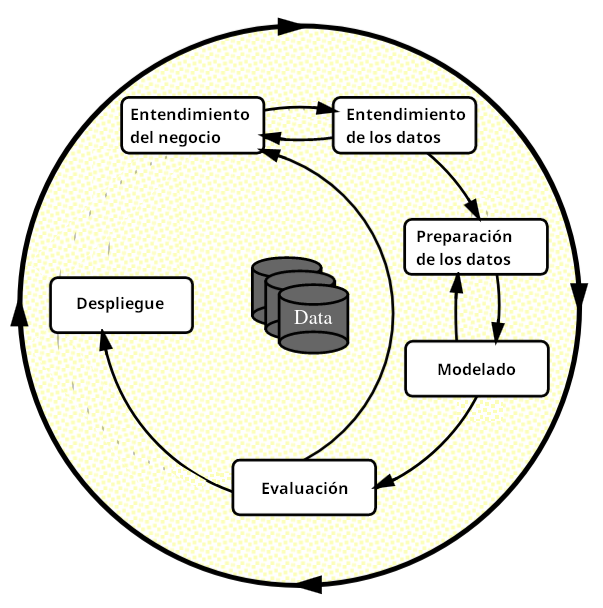
\includegraphics[width=0.6\textwidth]{herramientas_desarrollo/crisp-dm.png}
      \caption[CRISP-DM]{CRISP-DM \cite{wirth2000crisp}}\label{fig:herramientas_desarrollo/crisp-dm.png}
      \end{figure}
\FloatBarrier

\section{Herramientas de desarrollo}

Esta sección detalla las distintas herramientas, librerías y frameworks que
fueron utilizadas durante el desarrollo de este proyecto.

\subsection{Herramientas generales}

Estas herramientas han sido usadas para realizar tareas de forma general dentro
del proyecto.

\subsubsection{Fedora Linux}

Aunque al iniciar el proyecto se utilizó Windows 10 como sistema operativo
principal, la mayor parte del desarrollo ha sido realizado en la distribución de
Linux \href{https://fedoraproject.org/}{Fedora}, en concreto versiones 37 y 38.

Fedora se caracteriza por que sus repositorios se actualizan regularmente para
incluir las últimas versiones estables de la mayoría de programas, al contrario
de lo que ocurriría en una distribución como Debian estable. Pese a esto, Fedora
es considerada como una distribución bastante estable y, durante el desarrollo
de este proyecto, no se han encontrado problemas fuera de lo común.

Han sido instalados de forma nativa Python 3.9 para la fase de investigación,
\href{https://www.tug.org/texlive/}{\TeX{} Live} para la compilación de esta
documentación y \href{https://www.docker.com/}{Docker} para el desarrollo de la
aplicación web.

\subsubsection{Python}

Python es un lenguaje de programación diseñado con el objetivo de ser fácil de
escribir. Para lograr esto Python incluye de forma nativa una gran multitud de
funciones de uso común (como funciones de manipulación de cadenas), mientras que
en otros lenguajes debería encargarse el programador de implementarlas o
utilizar librerías de terceros. Esto tiene muchas ventajas, pero también algunas
desventajas, como, por ejemplo, que se pierde el control sobre la ejecución del
programa que podría dar un lenguaje como C o C++, lo que significa que, en
general, un mismo programa escrito completamente en Python va a ser más lento
que su contrapartida escrita en un lenguaje de programación de más bajo nivel en
el que se puedan especificar detalles como, por ejemplo, la gestión de memoria.

Pero Python tiene otra cualidad muy importante, y es su facilidad para
interactuar con código escrito en C o C++ mediante lo que se conoce como
\textit{bindings} o \textit{wrappers}. Esto permite al programador tener mayor
control sobre las partes más críticas de un programa, escribiéndolas en C por
ejemplo, mientras que las partes de menor importancia se pueden escribir
rápidamente en Python.

Un ejemplo perfecto de lo anterior es la librería
\href{https://github.com/numpy/numpy}{NumPy}, utilizada para la gestión de
matrices, entre muchas otras cosas. Esta librería implementa su funcionalidad
principal en C y expone una interfaz en Python para facilitar su uso.

Este patrón se repite una y otra vez en el campo del aprendizaje automático,
donde los algoritmos de aprendizaje se implementan a bajo nivel para que su
ejecución sea lo más rápida posible, mientras que se expone una interfaz a alto
nivel en Python para interactuar con los mismos. Ejemplos de esto son las
librerías \href{https://github.com/pytorch/pytorch}{PyTorch} y
\href{https://github.com/tensorflow/tensorflow}{TensorFlow}.

\subsubsection{Git}

Actualmente Git es el sistema de control de versiones más extendido en proyectos
de código abierto~\cite{OpenHubVCS}, en este proyecto se ha usado para gestionar
y guardar de forma segura los cambios que se han ido realizado con el tiempo en
la plataforma GitHub.

Aunque existen varias herramientas con interfaces gráficas que envuelven el
funcionamiento de Git (GitKraken, GitHub Desktop, etc.) para este proyecto se
utilizó directamente el comando \texttt{git} desde una terminal de Linux.

\subsubsection{Make}

A través del proyecto hay comandos de cierta complejidad que se repiten con
bastante frecuencia (\textit{e.g.} formatear el código, lanzar contenedores,
limpiar contenedores, etc.), para facilitar el uso de estos comandos se ha
utilizado la utilidad GNU Make, que viene por defecto en la mayoría de los
sistemas operativos de tipo Linux y se puede instalar tanto en Windows como en
MacOS.

El funcionamiento de Make consiste en la creación de un archivo denominado
\texttt{Makefile} que contiene diferentes comandos y secuencias de comandos con
las dependencias que existen entre los mismos.

Por ejemplo:

\begin{verbatim}
format:
    autoflake src
    isort src
    black src
\end{verbatim}

Un fichero \texttt{Makefile} con el contenido anterior permite ejecutar el
comando \texttt{make format} (siempre desde el mismo directorio en el que se
encuentra \texttt{Makefile}) para ejecutar la secuencia de comandos denominada
\texttt{format}, que, en este caso ejecutará varios comandos para realizar un
formato del código.

\subsubsection{PyCharm}

PyCharm es un Entorno de Desarrollo Integrado (IDE) creado y mantenido por
JetBrains, una compañía que se dedica a crear software y cuyos productos más
representativos son multitud de IDEs para diferentes lenguajes de programación
(IntelliJ (Java), CLion (C y C++), GoLand (Go), etc.).

El objetivo de PyCharm es facilitar el desarrollo de aplicaciones que utilizan
Python y da soporte amplio tanto para los habituales ficheros \texttt{.py} como
para \texttt{.ipynb} (Jupyter Notebook).

En este proyecto PyCharm fue utilizado para esarrollar la librería PADDEL
durante la fase de investigación, que contiene el código de Python común a los
Notebooks de Jupyter utilizados durante la fase de investigación.

\subsubsection{Visual Studio Code}

Visual Studio Code (VS Code) es un editor de texto orientado al desarrollo
creado por Microsoft. Gracias a su gran extensibilidad es posible utilizarlo
cómodamente en casi cualquier escenario.

Fue utilizado en la creación de esta documentación en conjunto con la extensión
\href{https://github.com/James-Yu/LaTeX-Workshop}{\LaTeX{} Workshop} que integra
distintos compiladores de \LaTeX{} (pdfTeX, XeTeX, LuaTeX, etc.) dentro del
programa y añade otras funcionalidades que hacen trabajar \LaTeX{} mucho más
conveniente.

Además, gracias a la extensión
\href{https://marketplace.visualstudio.com/items?itemName=ms-vscode-remote.remote-containers}{Dev
Containers}, VS Code puede ser lanzado desde contenedores de Docker, permitiendo
interactuar con las utilidades del contenedor. Gracias a esto VS Code ha sido la
herramienta utilizada para desarrollar por completo la aplicación web.

\subsubsection{Formateado de código Python}

Se han utilizado las siguientes herramientas para realizar el formateado del
código escrito en Python de forma automática:

\begin{itemize}
      \item \textbf{Autoflake}: herramienta utilizada para la eliminación de
            sentencias \texttt{import} y variables innecesarias.
      \item \textbf{Isort}: herramienta para la reordenación de sentencias
            \texttt{import}.
      \item \textbf{Black}: formateador de código caracterizado por un enfoque
            en convenciones, por esto permite una configuración muy limitada por
            parte del usuario.
\end{itemize}

\subsection{Herramientas para la fase de experimentación}

Estas herramientas han sido de gran utilidad durante la fase de experimentación
para realizar las distintas tareas como extracción de características y
entrenamiento de modelos.

\subsubsection{Jupyter Notebook}

Jupyter Notebook es una herramienta que permite crear un archivo con extensión
\texttt{.ipynb}, en el que el código Python se divide en ``celdas'' que se
pueden ejecutar individualmente, pero manteniendo y compartiendo las variables
establecidas de forma global entre todas estas celdas.

Esta herramienta fue de especial utilidad durante la fase de experimentación,
ya que permite observar detenidamente los cambios que se producen entre celdas
y, así, encontrar problemas sin tener que ejecutar el código completo desde el
principio cada vez que se realice un cambio, como ocurriría con un
\textit{debugger}.

Además de lo anterior Jupyter Notebook permite documentar de forma clara el
código mediante otro tipo de celda, en el que se puede escribir código en
Markdown, que es, en cierto modo, una alternativa menos verbosa a HTML.

\subsubsection{OpenCV}

OpenCV es una librería de visión artificial que contine varias utilidades para
interactuar con archivos de vídeo e imágenes de forma similar a como se
trabajaría en un programa como MATLAB\@. OpenCV está escrito en C y C++ pero tiene
\textit{bindings} que permiten interactuar con sus interfaces desde Python.

En este proyecto se usa para leer y decodificar los archivos de vídeo utilizados
durante la fase de investigación.

\subsubsection{MediaPipe}

MediaPipe es una librería de aprendizaje automático mantenida por Google que da
acceso a varios modelos preentrenados que se centran en la detección de
características corporales a partir de flujos de imágenes, en este caso se
utilizó MediaPipe Hands \cite{zhang2020mediapipe}, cuyo objetivo es extraer
varios puntos que definen un esqueleto ligeramente simplificado de la mano
humana.

\begin{figure}[H]
      \centering
      \subfloat{
\includegraphics[width=0.33\textwidth]{herramientas_desarrollo/mano.jpg}}
      \subfloat{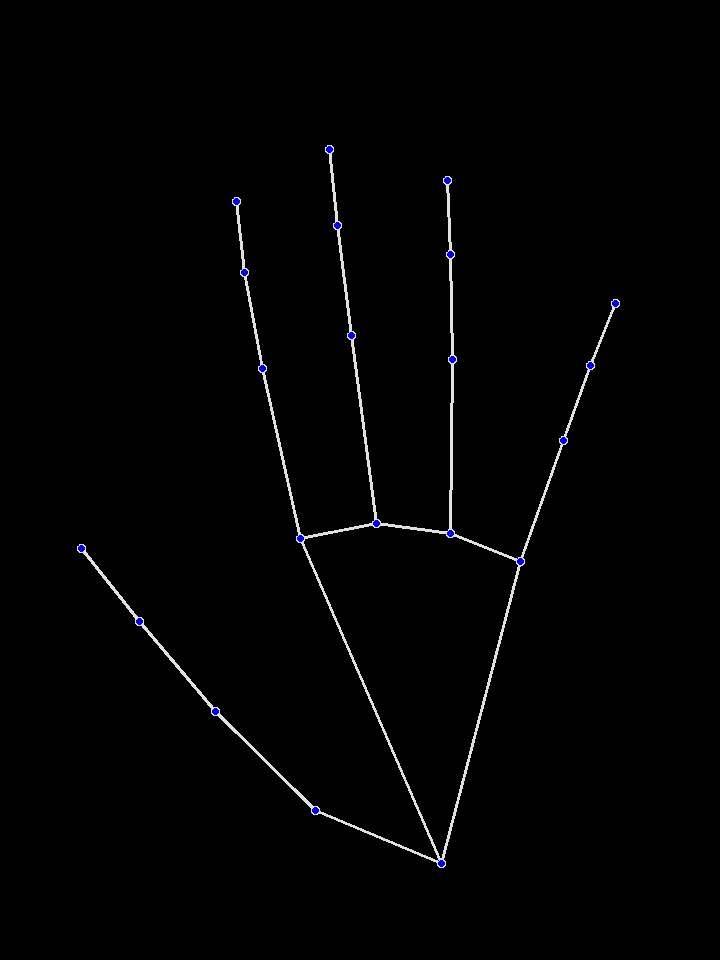
\includegraphics[width=0.33\textwidth]{herramientas_desarrollo/pose.jpg}}
      \subfloat{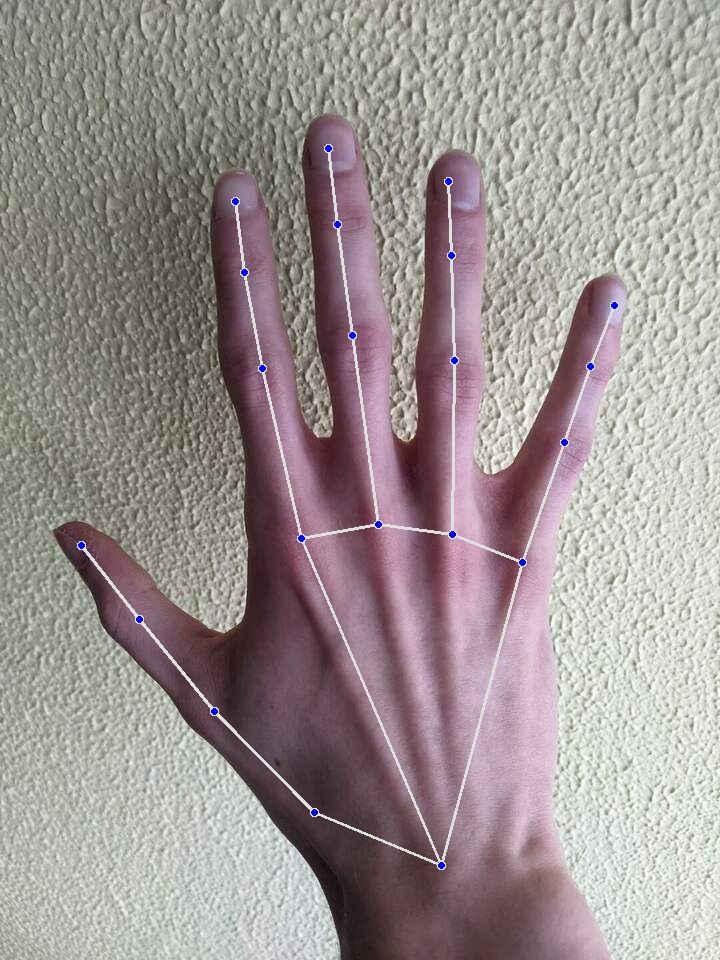
\includegraphics[width=0.33\textwidth]{herramientas_desarrollo/mano_pose.jpg}}
      \caption{MediaPipe Hands}
\end{figure}

Como se puede ver el resultado es bastante bueno, además, al utilizar vídeos
MediaPipe utiliza la información de los fotogramas anteriores para determinar de
forma más exacta la pose en los fotogramas posteriores. Esto es muy útil para
mejorar la precisión de las poses obtenidas, pero tiene la pega de que, al
necesitar información de pasos previos, el proceso de extracción de poses no se
puede paralelizar.

\subsubsection{TSFresh}

\href{https://github.com/blue-yonder/tsfresh}{TSFresh} \cite{christ2018time} es
una librería de Python que se encarga del preprocesado y la extracción de
características de series temporales.

Una serie temporal es una secuencia ordenada de valores con una componente
temporal asociada. Estas secuencias por sí solas no son de mucha utilidad para
entrenar algunos modelos, por lo que en la fase de preprocesado se debe realizar
una extracción de características sobre las mismas y así obtener características
numéricas que sí se pueden utilizar para entrenar un modelo.

TSFresh establece una forma estándar para extraer estas características,
permitiendo extraer características propias además de las, aproximadamente, 700
características que extrae por defecto.

\subsection{Herramientas para el desarrollo de la aplicación}

Estas utilidades fueron usadas para crear la aplicación web que se encuentra en
\href{https://paddel.catalin.sh}{paddel.catalin.sh}.

\subsubsection{Docker}

Docker permite la creación y gestión de contenedores, un contenedor se puede ver
como un sistema operativo dentro del anfitrión, pero sin llegar a ser una
máquina virtual, debido a que se utiliza el \textit{kernel} de Linux del sistema
anfitrión y los archivos del contenedor existen en el sistema de archivos del
anfitrión. Esto hace que la diferencia de rendimiento entre utilizar un
contenedor y ejecutar programas de forma nativa sea mínima.

Un contenedor de Docker se basa en lo que se conoce como una imagen, que es un
sistema de archivos preconfigurado para el propósito del contenedor. Se puede
encontrar una gran cantidad de imágenes en \href{https://hub.docker.com/}{Docker
Hub}, como, por ejemplo, postgres, node o python que ya incluyen los ejecutables
para utilizar cada herramienta respectiva. Sin embargo, es posible que se
necesite mayor control sobre la configuración de la imagen sobre la que se va a
construir el contenedor, en estos casos se pueden utilizar lo que se conoce como
\textit{Dockerfile} para crear una imagen tomando como base otra imagen ya
existente.

Un \textit{Dockerfile} es un archivo que determina la imagen de base a utilizar
(cualquier imagen de \href{https://hub.docker.com/}{Docker Hub} u otros sitios)
y los comandos a ejecutar para crear la imagen que se desea obtener. Si se
desease empezar de cero se puede utilizar una imagen de Ubuntu o Debian como
base.

Además de \textit{Dockerfile} existe otro tipo de archivo denominado
\textit{docker-compose.yml} utilizado para coordinar sistemas compuestos por
múltiples contenedores que interactúan entre sí. La aplicación web de este
proyecto utiliza \textit{docker-compose.yml} para determinar las interacciones
entre los cuatro contenedores creados (web, API, proxy inverso y base de
datos).

\subsubsection{Caddy}

En las fases iniciales de desarrollo se decidió que la API debería estar alojada
en el subdominio \texttt{api.}, mientras el dominio principal debería llevar a
la web (SvelteKit). Esto significa que van a existir dos servicios funcionando
de forma paralela (Web y API), y que dependiendo del dominio al que se realice
una petición, ésta debería ser redirigida a un servicio u otro.

Esta situación es uno de los casos de uso idóneos para un proxy inverso, que es
un servicio que recibe peticiones HTTP, las altera si es necesario, y las
redirige al servicio de destino (el cual se determina mediante ciertas reglas de
redirección).

En un principio se optó por utilizar Nginx para implementar este proxy inverso
con muy buenos resultados gracias a su fácil configuración, rendimiento y
simplicidad. Pero surgieron problemas al añadir soporte para utilizar
certificados SSL y realizar peticiones seguras mediante HTTPS, ya que era
deseable una solución que gestionase de forma automática la petición y
renovación de estos certificados y Nginx, debido a su simplicidad no dispone de
esta funcionalidad.

Se probaron dos alternativas que solucionaban este problema, Traefik y Caddy,
ambas escritas en GoLang. Traefik dispone de una gran cantidad de
funcionalidades incluyendo gestión de certificados SSL, entre muchas otras, como
un panel de control desde el que visualizar estadísticas sobre el nivel de uso
del servicio.

La otra alternativa, Caddy, es mucho más simple, pero realiza la gestión de
certificados de forma automática por defecto, e incluso permite el uso de
certificados \textit{self-signed} (firmados por uno mismo, en lugar de por una
entidad certificadora). Esto es de gran utilidad durante el desarrollo para
asegurar que el funcionamiento de la aplicación va a seguir siendo el mismo en
el entorno final de producción (ya que hay ligeras diferencias dependiendo de si
un navegador utiliza HTTP o HTTPS).

Es por todo lo anterior que, en última instancia, se decidió usar Caddy.

\subsubsection{FastAPI}

FastAPI es un \textit{framework} de Python utilizado para crear APIs de tipo
REST que se caracteriza por permitir al programador centrar sus esfuerzos en el
código relacionado con la lógica de negocio al realizar la mayoría de las
acciones comunes entre diferentes APIs por defecto (como la creación de
documentación, validación de tipos, serialización y deserialización de
peticiones, etc.).

En este proyecto se ha creado una API REST para permitir la interacción con el
código de Python utilizado para crear, entrenar y utilizar los modelos desde
cualquier dispositivo y lenguaje de programación (siempre y cuando permita
realizar peticiones HTTP). Con esto se consigue que en el futuro se puedan crear
nuevas formas para interactuar con los modelos sin necesidad de alterar el
código ya existente. Se podría, por ejemplo, crear una aplicación móvil para
facilitar la toma y subida de vídeos. Además, estas nuevas aplicaciones podrían
estar creadas por personas ajenas al proyecto que necesiten una implementación
diferente para su caso de uso específico.

\subsubsection{SvelteKit}

Para el frontend de la aplicación, es decir, todo lo que va a ver un usuario de
la web (HTML, CSS y JavaScript), se ha utilizado
\href{https://kit.svelte.dev/}{SvelteKit}, que es un framework de JavaScript
basado en Svelte. Es similar a otros frameworks más populares como React o
Angular, y se caracteriza por tener una sintaxis muy clara y simple además de
reducir el tamaño de los archivos que se envían al navegador del cliente,
haciendo que, en general, las páginas creadas con SvelteKit sean más rápidas que
sus contrapartidas.

\subsubsection{Typescript}

JavaScript es un lenguaje de programación que no dispone de tipado estático, lo
cual hace muy difícil detectar problemas fuera del tiempo de ejecución.

\href{https://www.typescriptlang.org/}{TypeScript} es un lenguaje de
programación desarrollado por Microsoft que utiliza una sintaxis de base muy
similar a la de JavaScript, pero añadiendo tipado estático. Los navegadores no
``entienden'' TypeScript, por lo que éste debe ser compilado a JavaScript antes
de ser enviado al usuario. Durante esta compilación se pueden detectar multitud
de errores gracias al tipado.

\subsubsection{Typesafe i18n}

\href{https://github.com/ivanhofer/typesafe-i18n}{Typesafe i18n} es una librería
escrita en TypeScript que se puede utilizar para internacionalizar aplicaciones
web, es decir, añadir soporte para más idiomas, de forma simple y mediante unas
convenciones predefinidas.

Para ello se crea un archivo para cada idioma al que se de soporte, en el que se
definen las variables con las cadenas de texto utilizadas a través de la web en
el idioma respectivo. Cada uno de estos archivos debe contener las mismas
variables.

A continuación, en los lugares donde se usen cadenas de texto se debe importar la
variable \texttt{LL} que es un objeto con todas las traducciones que se puede
usar en la página respectiva para establecer las cadenas de texto dependiendo
del idioma.

\subsubsection{Axios}

\href{https://github.com/axios/axios}{Axios} es una librería de JavaScript que
envuelve la función nativa \texttt{fetch} para hacerla más amigable y fácil de
usar. Se caracteriza por soportar tipos de TypeScript y simplificar la
realización de peticiones HTTP.

En este proyecto se ha utilizado esta librería para realizar peticiones REST a
la API desde el navegador del usuario. Para ello se han creado multitud de
funciones que reflejan los \textit{endpoints} de la API y, así, permitir su uso
desde el resto del sitio web.

\subsubsection{Tailwind CSS}

\href{https://tailwindcss.com/}{Tailwind CSS} es una librería de clases de CSS,
su funcionamiento es similar a \href{https://getbootstrap.com/}{Bootstrap} en
cuanto a que existen multitud de clases que realizan diferentes acciones. La
diferencia está en que Tailwind CSS es mucho más modular que Bootstrap, es
decir, las clases realizan cambios muy pequeños sobre los objetos a los que
afectan. Esto hace que Tailwind sea más lento de escribir que su contrapartida,
pero al mismo tiempo permite un nivel mucho mayor de configuración sobre el
diseño de una página web.

\subsubsection{Prettier}

\href{https://prettier.io/}{Prettier} es un formateador de código, creado
concretamente para dar un formato consistente a archivos de HTML, CSS,
JavaScript, TypeScript, etc.

\subsubsection{ChromeVox}

Un aspecto que se tuvo muy en cuenta durante el desarrollo del sitio web es la
accesibilidad, en especial para usuarios con visibilidad reducida que dependen
de lectores de pantalla para descubrir el contenido de la web.

Para comprobar cómo interactuaría un lector de pantalla con la aplicación se ha
utilizado la extensión de Google Chrome
\href{https://chrome.google.com/webstore/detail/screen-reader/kgejglhpjiefppelpmljglcjbhoiplfn}{ChromeVox}.
